\documentclass[twocolumn,superscriptaddress,aps]{revtex4-1}

\usepackage[utf8]{inputenc}

\usepackage{amsfonts}
\usepackage{amssymb}
\usepackage{amsmath}
\usepackage{amsthm}
\usepackage{float}

\usepackage{bbold}
\usepackage{bm}
\usepackage{color}
\usepackage{hyperref}
\usepackage{graphicx}
\graphicspath{{figures/}}

\begin{document}


% ==============================================================================

\title{\Large{INFO8010: Brain Cancer Detection Project Report}}
\vspace{1cm}
\author{\small{\bf Ayoub Assaoud}}
\affiliation{\texttt{ayoub.assaoud@student.uliege.be} (\texttt{s207227})}

\maketitle
\section{Abstract}

\section{Introduction}
%%% Introduction: which states the problem which has been tackled

For this project we propose to build a generative deep learning system that can generate anime faces. The system will be trained on a dataset of anime faces and will use denoising diffusion probabilistic models (DDPM) to generate new faces. The goal is to create a system that can generate acceptable quality anime faces that are diverse and realistic by drawing samples, and naturally for denoising by encoding-decoding the image. The project will also explore the use of different architectures and the impact of self-attention on standard DDPM to improve the quality of the generated faces.

Through this project, we:

\begin{itemize}
	\item Collecte and preprocess over than 80,000 anime face images, applying normalization, resizing, and few augmentations.
	\item Design and train two distinct deep learning models, mainly noise prediction technique and have a quick view on score-based energy model, experimenting with different architectures and training strategies.
	\item Evaluate performance using some basic metrics.
\end{itemize}
In the following sections, we'll walk through related work, our data pipeline, model Architecture, and results.

\section{Related Work}
%%% Related Work: which covers research that is related to the considered problem
\subsection{Denoising Diffusion Probabilistic Models}

Denoising Diffusion Probabilistic Models (DDPM), introduced by Ho et al.~\cite{ho2020ddpm}, laid the foundation for a class of generative models that iteratively reverse a diffusion process to synthesize high-quality data samples. The original DDPM framework employs a convolutional U-Net architecture to model the denoising function, demonstrating impressive results in image generation without relying on attention mechanisms.

Subsequent works have extended this paradigm by integrating transformers to better capture long-range dependencies and enable multimodal conditioning, particularly in text-to-image synthesis tasks. Models such as GLIDE~\cite{nichol2021glide}, Imagen~\cite{saharia2022imagen}, and DALL·E 2~\cite{ramesh2022hierarchical} exemplify this shift, incorporating transformer-based components to enhance expressiveness and scalability.

Our work builds on this trajectory by exploring the role of transformers within the DDPM framework, aiming to enhance diffusion modeling with the representational power of attention-based architectures, as well as discussing some limitations and choices.

\subsection{Modified Forward Diffusion Kernel}
Recent efforts have explored modifications to the forward diffusion kernel in DDPMs to improve sampling efficiency and image quality. The LearnOpenCV guide~\cite{learnopencv2023ddpm} discusses a variant where the noise schedule and kernel are adapted to better preserve semantic structure during the forward process. By refining the way noise is injected, this approach aims to maintain more meaningful latent representations, which in turn facilitates more accurate denoising during reverse diffusion.

Such kernel-based modifications offer a promising direction for enhancing DDPMs without fundamentally altering their probabilistic framework. Our work complements these ideas by investigating how transformer-based architectures can further improve the expressiveness and flexibility of the denoising model.

% \href{https://learnopencv.com/denoising-diffusion-probabilistic-models/#modified-forward-diffusion-kernel}{Modified Forward Diffusion Kernel}

\section{Methods}
%%% Methods: a clear and detailed description of the neural networks (architecture, training-parameters, loss function, data)
\subsection{Data}
\begin{figure}[htbp]
	\centering
	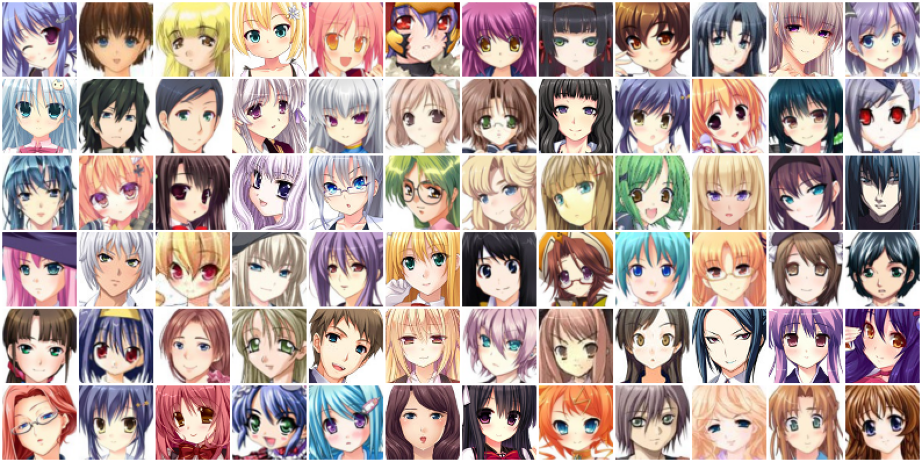
\includegraphics[width=0.5\textwidth]{figures/original_data_samples_grid.png}
	\caption{Images from the anime faces dataset.}
	\label{Figure 1: dataset}
\end{figure}
\subsubsection{Dataset Description}

we took the \href{https://www.kaggle.com/datasets/splcher/animefacedataset/}{\textbf{Anime Face Dataset}} ($63k$ images), in addition to \href{https://www.kaggle.com/datasets/soumikrakshit/anime-faces}{\textbf{soumikrakshit Anime Face}} ($21k$ images).


\subsubsection{Data Preprocessing}
Our preprocessing pipeline was implemented in Python using PyTorch library, and included the following steps:

\begin{itemize}
	\item \textbf{Cleaning}: To insure a better quality of dataset, we removed all images for which the size is less than 64x64, resulting in 80k remaining images.
	\item \textbf{Resizing:} All images were resized to a fixed size of 64x64 pixels.
	\item \textbf{Normalization:} We normalize the pixel values to the range [-1, 1], to keep consistent with the noise distribution. an it seems to be much more effective than constraining the model to output values in the [0, 255] range, as it allows for better training stability and convergence.
	\item \textbf{Data Augmentation:} We applied random horizontal flipping, no rotation or cropping was applied because most faces were not centered, or touching the frame which could lead to poor generated samples.
\end{itemize}


\subsubsection{Spliting Data:}\label{split_data}
We split the dataset into training set and validation set, with a ratio of 90:10, althought this splitting is not strictly necessary for DDPMs, and not that significant than it could be for classification tasks, we still did it to have at least an idea about the model's denoising performance on unseen data.

%%%%%%%%%%%%%%%%%%%%%%%%%%%%%%%%%%%%%%%%%%%%%%%%%%%%%%%%%%%%%%%%%%%%%%%%%%%%%%%%%%%%%%%
\subsection{Architecture}
The denoising diffusion probabilistic model (DDPM) consists of a forward diffusion process that progressively adds gaussian noise to the data, and a reverse diffusion process that learns to denoise the data. This architecture allows for high-quality image generation by sampling from the a known distribution $q(x_T) \sim \mathcal{N}(0, I)$ then gradually denoising at each step with our model.

the same architecture can be used to approximate the score function of the data distribution $s_\theta(x , t) \approx \nabla \log p_t(x_t)$.

\subsubsection{Description of the general architecture for the denoiser model}

\begin{itemize}
	\item \textbf{U-Net:} A U-Net architecture is used as the denoiser model that predicts the original noise $\epsilon \approx\epsilon_\theta(x_t, t)$ for the DDPM.
	\item \textbf{ResNet Blocks:} We incorporate residual blocks to improve the flow of gradients during training, which helps in learning complex features, thanks to skip connections.
	\item \textbf{Attention Mechanisms:} We incorporate attention mechanisms to improve the model's ability to focus on relevant features during the denoising process.
\end{itemize}

The Unet architecture consists of Three main components: a chain of $len(down_channels)$ \textbf{DownEncoder}, a chain of $len(mid_channels)$ \textbf{Bottleneck}, and a chain of $len(down_channels)$ \textbf{UpDecoder}, to preserve symmetric feature mapping.

The \textbf{DownEncoder} reduces the spatial dimensions (H,W) of the input image while increasing the number of feature channels, which is called downs ampling, allowing the model to learn hierarchical representations.

The \textbf{Bottleneck} connects the DownEncoder and UpDecoder, serving as a bridge that captures the most abstract features.

The \textbf{UpDecoder} then reconstructs the image by progressively increasing the spatial dimensions while reducing the number of feature channels (up sampling) and concatenates the correspondding levels DownEncoder outputs with those of the UpDecoder.

Each of these subcomponents is composed of a number of \small{$ModelParams.num\_(down\|mid\|up)\_layers$} \textbf{block layers}, each of these block layers consists of a stack of ResNet block followed by a self-attention layer (optional in our case see discussion) and finally an optional convolutive layer (downsampling or upsampling), see figure bellow.

% \footnote{this expression means either \small{$ModelParams.num\_(down\|mid\|up)\_layers$}}
\begin{figure*}[ht]
	\centering
	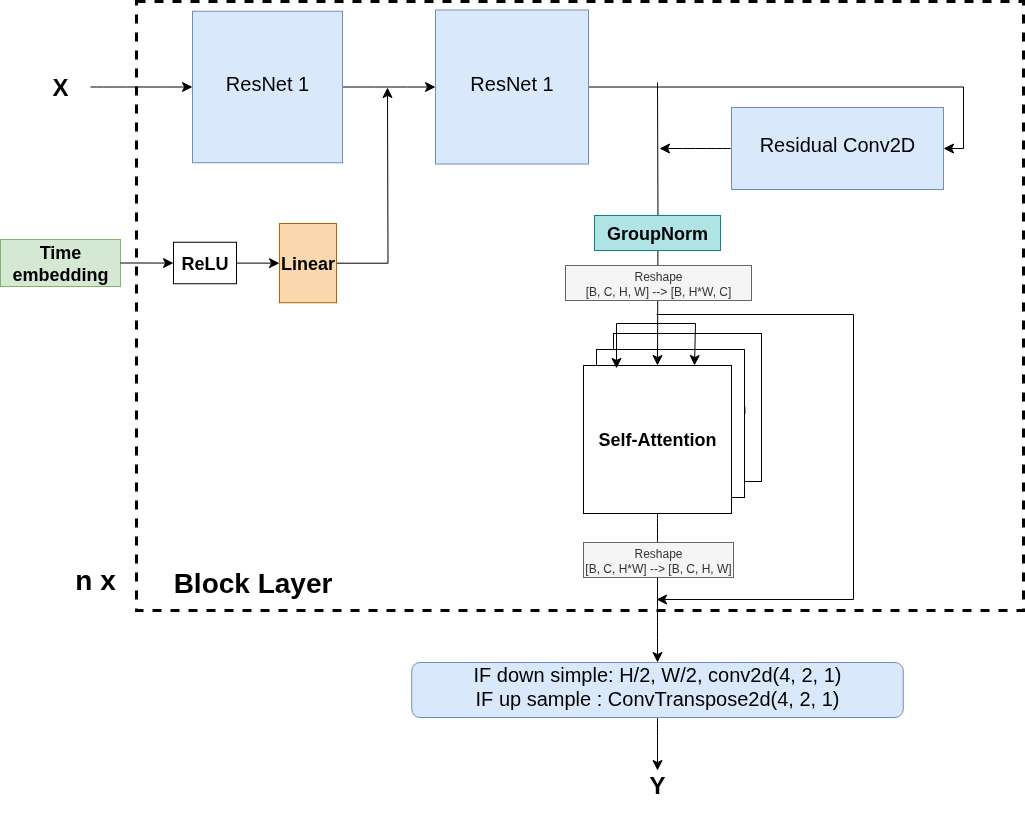
\includegraphics[width=0.8\textwidth]{figures/block_layer.png}
	\caption{Block layer Architecture with ResNet blocks and self-attention layers, depending on the subcomponent, the number n is equal to \small{$ModelParams.num\_(down\|mid\|up)\_layers$}}
	\label{fig:unet_architecture}
\end{figure*}

The ResNet block consists of two convolutional layers with Group normalization and SiLU activation, allowing the model to learn residual mappings, and the input is added to a \textbf{positional embedding learnable vector} after the first convolutional layer, whereas the self-attention layer allows the model to focus on relevant features in the input image, improving the quality of the generated images.

The DownEncoder uses strided convolutions to reduce the spatial dimensions, while the UpDecoder uses transposed convolutions to increase them. The Bottleneck uses standard convolutions without striding.


% %%%%%%%%%%%%%%%%%%%%%%%%%%%%%%%%%%%%%%%%%%%%%%%%%%%%%%%%%%%%%%%%%%%%%%%%%%%%%%%%%%%%%%%
\subsubsection{Motivating choices}

\textbf{the choice of activation function:} we chose SiLU (Sigmoid Linear Unit) as the activation function for the model, which is known to improve the flow of gradients and enhance the model's ability to learn complex features. SiLU has been shown to outperform ReLU in many cases, especially in image-tasks.
in other point of view, image pixels are normalized to the range [-1, 1], and the SiLU activation function is well-suited for this range, as it smoothly transitions between negative and positive values.
$SiLU(x) = x \cdot \sigma(x)$

\begin{figure}[ht]
    \centering
    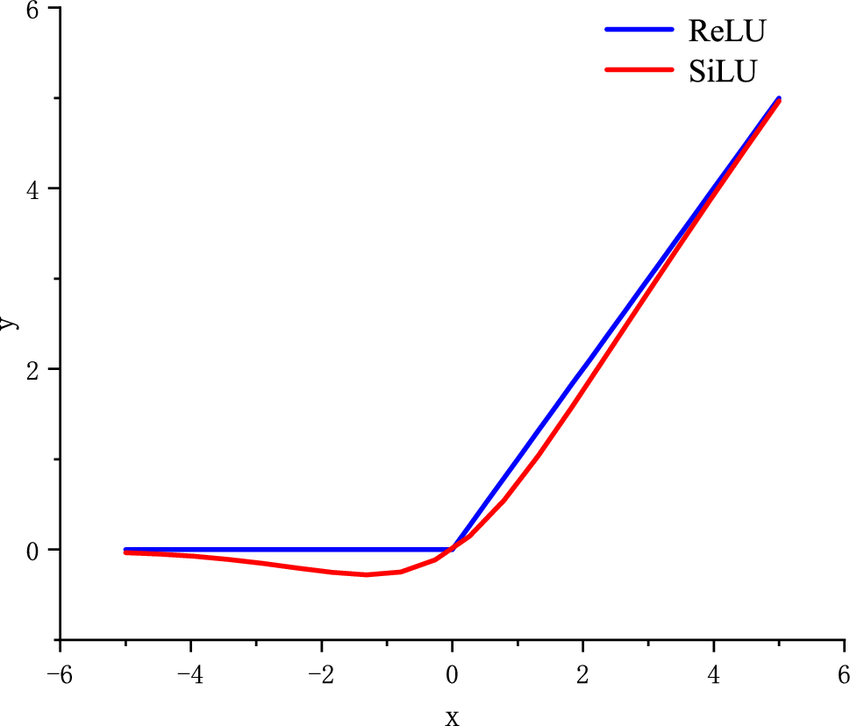
\includegraphics[width=0.3\textwidth]{figures/ReLU-and-SiLU-activation-function-curve.png}
    \caption{SiLU and ReLU Activation Functions, from \small{\href{https://www.researchgate.net/figure/ReLU-and-SiLU-activation-function-curve_fig1_363232692}{www.researchgate.net}} }
    \label{fig:silu}
\end{figure}


\textbf{the choice of normalization:} we used Group Normalization instead of Batch Normalization, to normalize the features within groups independently from batches, which is more effective in stabilizing training, especially that in our cases batch size was set to 6, which is small, because we hit the GPU's Limit, it is also good for variable batch size while evaluation.

\textbf{the choice of attention mechanism:} as modern architectures often incorporate attention mechanisms, we used self-attention layers to helps the model to capture long-range dependencies and relationships between pixels, which is crucial for generating high-quality images.

the shape of the input of self-attention is : $[B, H*W, C_i]$
respectively batch, height, weight and out\_channels of a given subcomponent. Which makes relationships between pixels more explicit than $[B, C_i, H*W]$, we explored the impact for this decision especially for Mega 74M model in the sections bellow.

this mechanism has an impact, as we will see in the comming sections, that there is a trade-off between an attention block for each block layer and the model's performance.
% as it increases the number of parameters, requires more data to train, sensible to noise...
% for remark, the impact of not having normalized data in the beginnd was poor sampling with dark images...
we will get a tour over the architecture we have tried in the order of their complexity.


\subsubsection{Recapitulative Table:}
It is important to mentionne that at the beginng, we took $[B, C_i, H*W]$ as the input shape for attention, and the stratigy to enhance performance was to increase the capacity by increasing stages of DownEncoder and UpDecoder, as well as the number of block layers in each subcomponent, but it was not effective, thus we changed the input shape to $[B, H*W, C_i]$ and we tried to increase the capacity by increasing the number of channels in DownEncoder and UpDecoder, as well as the number of block layers in each subcomponent.
\begin{table}[ht]
\centering
    \begin{tabular}{|lc|cc|c|c|c|c|}
    \hline
        \rotatebox{90}{\textbf{Model Name}} & \rotatebox{90}{\textbf{Params (M)}} & \rotatebox{70}{\textbf{Down Channels}} & \rotatebox{90}{\textbf{Down Layers}} & \rotatebox{70}{\textbf{Mid Channels}} & \rotatebox{90}{\textbf{Mid Layers}} & \rotatebox{90}{\textbf{Attention}} & \rotatebox{90}{\textbf{Time Emb Size}} \\
        \hline
        mini   & 10 & [32,64,128,256]     & 2 & [256,256,128] & 2 & \small{full}    & 128 \\
        Simple & 49 & [32,64,128,256,512] & 3 & [512,512,256] & 2 & \small{full}    & 128 \\
        Mega   & 74 & [32,64,128,256,512] & 5 & [512,512,256] & 3 & \small{full}    & 128 \\
        Giga   & 85 & [128,256,256,512]   & 5 & [512,512,256] & 5 & \small{partial} & 128 \\
        \hline
    \end{tabular}
    \label{tab:architecture_parameters}
\caption{Model architecture parameters for each model.}
\end{table}

NB: $down\_channel = up\_channels$

\subsubsection{Mini U-Net DDPM 10M Architecture:}
\paragraph[short]{Bad Attention Input Shape: $[B, C_i, H*W]$}
we use $[B, C_i, H*W]$ as input shape for attention, it never generate a face, producing some noisy mono-color backgrounds, with a 2 little dark (eyes-like) stains, then it continiousely decreading quality until generating uncomprehensive noise with almost the same grade of colors.

Its best (still poor) performence is reached in first epochs. However, is was remarked that the model is still denoising validation set fairly enough.

\begin{figure}[H]
    \centering
    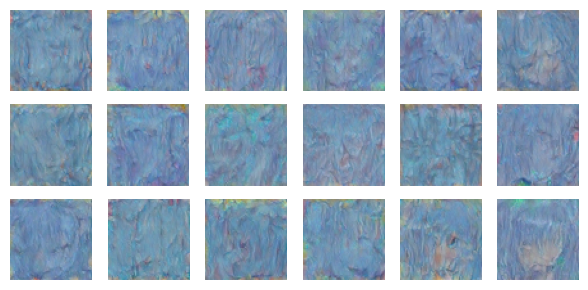
\includegraphics[width=0.3\textwidth]{figures/10M_epoch5_slightely diff_cains_bad_attention_.png}
    \caption{Samples from Mini U-Net DDPM 10M Architecture at epoch 5 with bad attention.}
    \label{fig:10M_epoch5_slightely_diff_cains_bad_attention_}
\end{figure}


\paragraph[short]{Good Attention Input Shape: $[B, H*W, C_i]$}
The idea is to know weither we can reach an acceptable quality of the images, strictely increasing down channels in the DownDecoder, with attention in each block layer.

the model is not capable of generating coherent sampled images in the first epochs, its best performence is reached at the 15th epoch, but some regions in the latent space $x_T$ are empty or under-represented, such that we obtain some images with the same color, some images that are identical to original data, which indicates that model is overfitting and begins to collapse withour being capable to generalize. but the model is still denoising fairly good as larger models.
\begin{figure}[H]
    \centering
    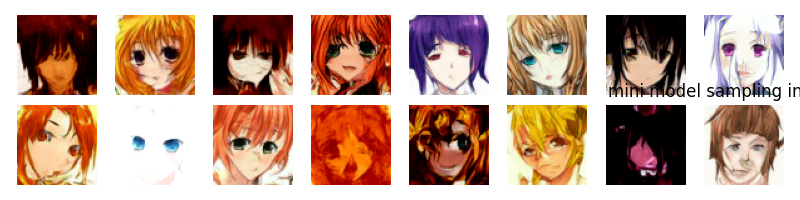
\includegraphics[width=0.4\textwidth]{figures/mini_unet_ddpm_10M_ckpt_epoch_15_epoch_15_samples.png}
    \caption{Samples from Mini U-Net DDPM 10M Architecture at epoch 15.}
    \label{fig:mini_unet_ddpm_10M_ckpt_epoch_15_epoch_15_samples}
\end{figure}
Having less empty images may indicated that latent variable space is compact, in other words, the model is learning a more structured representation of the data, which can be due to its small capacity, but we aim a better results.

\subsubsection{Simple U-Net DDPM 49M Architecture:}
the second try was to augment the capacity of the model by increasing the number of block layers to 3 and an additional layer of DownEncoder (automatically UpDecoder) to reach 512 channels, while preserving the good input shape.

the performence has increased, but the sampling quality is still poor and not diverse, some samples are either white or black backgrounds, and struggles to generalize even after many epochs. 
%reachs the best performance in the 3th epochs, an continues with the same assumptoms of previous one.
\begin{figure}[H]
    \centering
    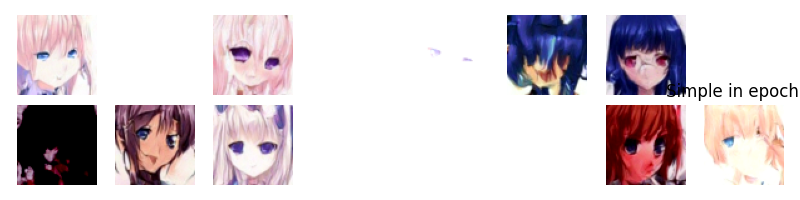
\includegraphics[width=0.4\textwidth]{figures/simple_unet_ddpm_49M_ckpt_epoch_13_2025-08-14_12-52-58_epoch_13_samples.png}
    \caption{Samples from Mega U-Net DDPM 74M Architecture at epoch 13.}
    \label{fig:mega_unet_ddpm_74M_ckpt_epoch_13_epoch_13_samples}
\end{figure}

\subsubsection{Mega U-Net DDPM 74M Architecture:}
here we augment the capacity of the model by increasing the number of block layers of DownEncoder and UpDecoder to 5, Bottleneck to 3 layers.
% \paragraph[short]{Bad Attention Input Shape: $[B, C_i, H*W]$}
Feed attention mechanism with inputs of the shape $[B, C_i, H*W]$, which focuses on the relationships across channels instead of pixel-to-pixel relationships, resulted in bad performance. However, Mega was capable of generating some reasonable samples, but they were sharp, slightly noisy and poorly divergent.
\begin{figure}[H]
    \centering
    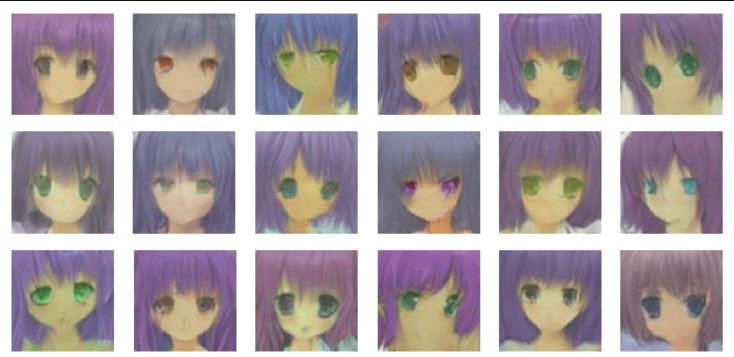
\includegraphics[width=0.3\textwidth]{figures/Screenshot from 2025-08-06 17-12-05.png}
    % \caption{Samples from Mega U-Net DDPM 74M Architecture at epoch 6.}
% \end{figure}
% fo
% \begin{figure}[ht]
    % \centering
    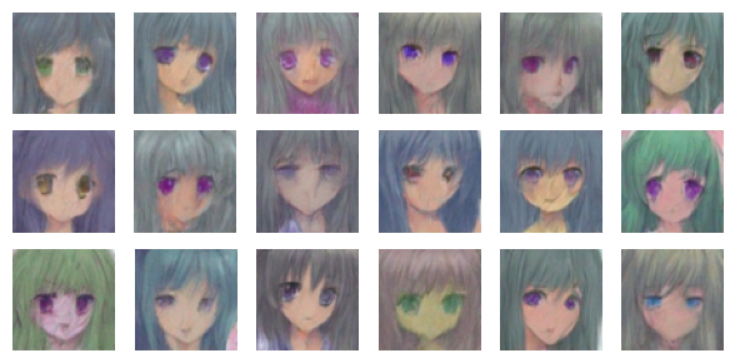
\includegraphics[width=0.3\textwidth]{figures/Screenshot from 2025-08-06 20-09-30.png}
    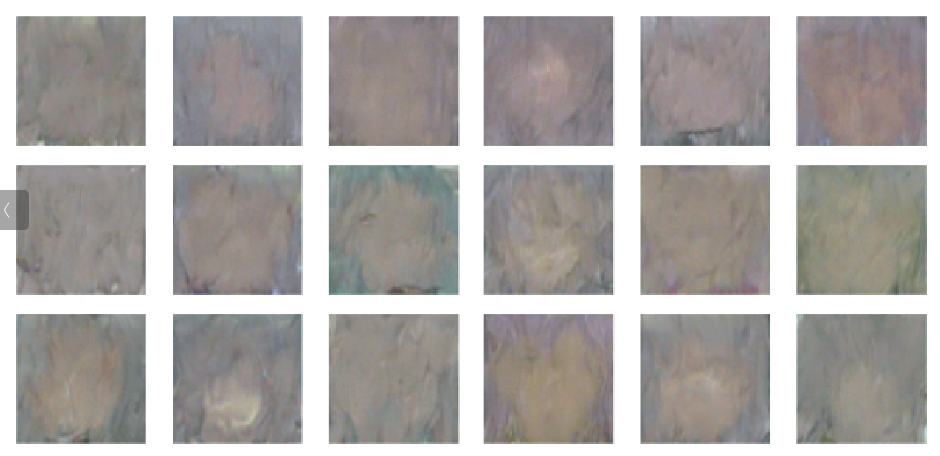
\includegraphics[width=0.3\textwidth]{figures/74M-badattention-epoch16.png}
    \caption{Samples from Mega U-Net DDPM 74M Architecture, bad input shape, at respectively 6, 8 and 16 epochs.}
\end{figure}


We notice that epochs between 5 and 9, every epoch has a common samples pattern, such as hair colors, face color, sharpness, the model stick to one pattern, similar faces, thus we beleive that attention mechanism has its role on this issue as well as the limited size of batch (2)\footnote{The same resource 2x(Nvidia a5000) allows training Mega on 2 batches, while allowing 6 batches for Giga.}.
then at later epochs, the model starts to generate pure noise with a fixed mean that corresponds to ebony.

Here it was the first trigger that shifted our approach to think about the architecture choices and specially input shape of attention, as we noticed that the model is not capable of generating diverse samples, and it seems to be stuck in a local minimum, which is a common issue in deep learning models, especially when the model is too complex or the data is not diverse enough.
% \paragraph[short]{Good Attention Input Shape: $[B, H*W, C_i]$}
% the result is an important improvement in the quality of samples, in epoch 13. but the results sill not that saisfactory, because there still some void images, slow learning and lack of diversity.

% , some darkness themes, lake of sharpness as well as some sort of noisy face patterns.



\subsubsection{Giga U-Net DDPM 85M Architecture:}
Here we decided to increase the capacity of the model by upgrading the size of channels to become $[128, 256, 256, 512]$, refer to table \ref{tab:architecture_parameters}, you will notice also that channels are increasing non strictly in the DownEncoder and UpDecoder, while keeping the same number of block layers to 5 for both DownEncoder and UpDecoder, and increasing to 5 for Bottleneck.

In addition, we decided that a transformer for each block layer may be not a good idea, as it requires too much data to train and more prone to noise, as well as for computaion limited ressource issues, thus in Giga model, we apply the attention layer as follows:

\begin{table}[h!]
	\centering
	\begin{tabular}{|c|c|c|c|c|c|}
		\hline
		\textbf{Layer} & \textbf{Pos 1} & \textbf{Pos 2} & \textbf{Pos 3} & \textbf{Pos 4} & \textbf{Pos 5} \\
		\hline
		Down           & False          & True           & False          & True           & True           \\
		Mid            & False          & True           & False          & -              & -              \\
		Up             & False          & True           & False          & True           & False          \\
		\hline
	\end{tabular}
	\label{tab:attention_application}
	\caption{Attention application across Block layers}
\end{table}
% down_apply_attention: list = (False, True, False, True, True)
% mid_apply_attention: list = (False, True, False)
% up_apply_attention: list = (False, True, False, True, False)
Such that the first block layer does not contain an attention layer, the idea is to obtain some meaningful input for the transformer, our best-choice is inspired from GPT, BERT and modern Large languages models that take as input a meaningful semantic vectors from pretrained embedding technologies like word2vec, FastText..., then passes through a transformer-based encoder/decoder block.

Thus we do the same thing for images, but with convolution-oriented layers (such ResNet) that tend to extract meaningful features from images, to feed them to our self-attention layers within the block layer.

Let us take an overview on the samples generated by Giga model in the first epochs.
\begin{figure}[H]
    \centering
    \begin{tabular}{c}
        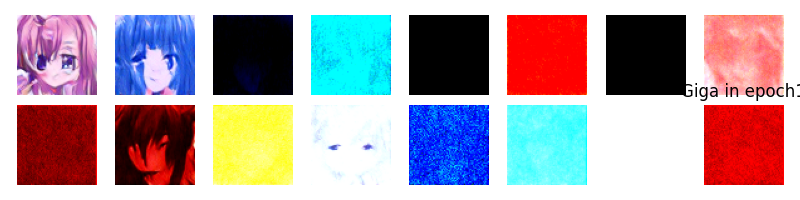
\includegraphics[width=0.5\textwidth]{figures/85M_params_GIGA_DDPM_Unet_ckpt_epoch_1_epoch_1_samples.png}\\\hline
        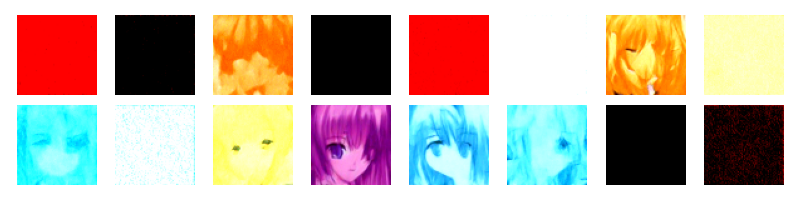
\includegraphics[width=0.5\textwidth]{figures/85M_params_GIGA_DDPM_Unet_ckpt_epoch_3_with_16_samples.png}\\\hline
        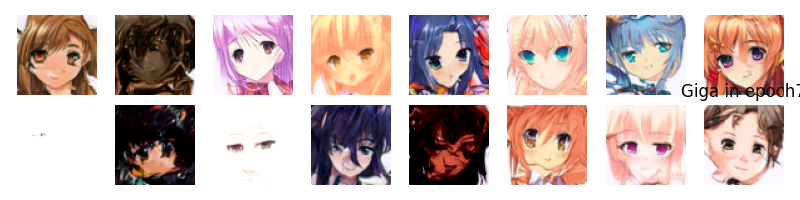
\includegraphics[width=0.5\textwidth]{figures/85M_params_GIGA_DDPM_Unet_ckpt_epoch_7_epoch_7_samples.png}\\\hline
        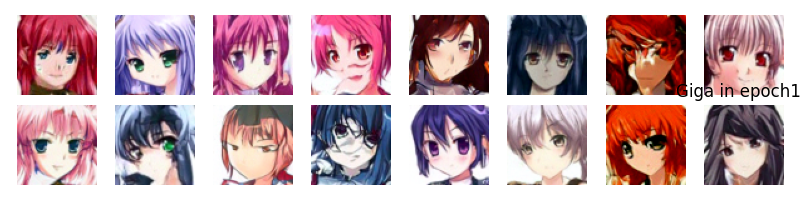
\includegraphics[width=0.5\textwidth]{figures/giga_unet_ddpm_85M_ckpt_epoch_10_epoch_10_samples.png}\\\hline
        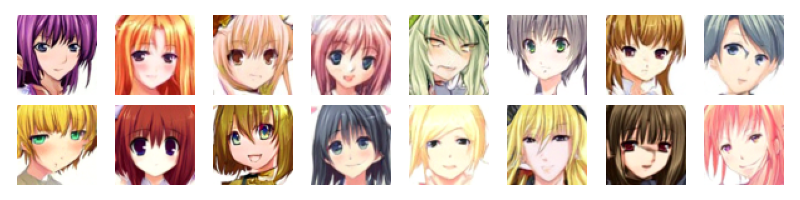
\includegraphics[width=0.5\textwidth]{figures/giga_unet_ddpm_85M_ckpt_epoch_17_with_16_samples.png}\\\hline
        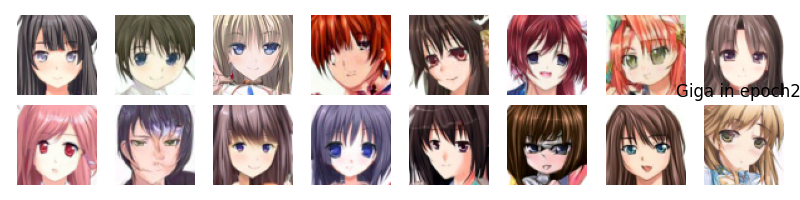
\includegraphics[width=0.5\textwidth]{figures/giga_unet_ddpm_85M_ckpt_epoch_22_epoch_22_samples.png}
    \end{tabular}
    \caption{Samples from Giga U-Net DDPM 85M Architecture respectively after 1, 3, 7, 10, 17 and 22 epochs.}
    \label{fig:giga_unet_ddpm_85M_ckpt_epoch_3_epoch_3_samples}
\end{figure}

We can see that the model is capable of generating coherent faces, with diversity, while impresively achieving the same performance for smaller models in even earlier epochs.

It also produces cleaner images even in the earlier epochs in comparison with Mega 74M model, which is not the case with smaller models that contains full transformer.

% Earliest epochs produce more diversity, and coherent faces which means that

We believe that this significant improvement is not only due to the capacity of the model given the additional 10M parameters, but also to the change of the architecture, notably by omitting some attention layers in the early stages, as well as allowing for bigger batch sizes (at most 6) which lead to a stability  in training, which can be seen in the train and validation loss plots in the next section.

What was also surprising is the fact that the model is capable of generating coherent faces very early, which was not the case with smaller models, and it seems to be more stable during training, as we can see in the train and validation loss plots.


% %%%%%%%%%%%%%%%%%%%%%%%%%%%%%%%%%%%%%%%%%%%%%%%%%%%%%%%%%%%%%%%%%%%%%%%%%%%%%%%%%%%%%%%
\subsection{Training}

Our training technique is based on standard denoising diffusion probabilistic models (DDPM) paper. we trained the model to predict the original noise $\epsilon$ given a noisy image $x_t$ and a time step $t$. The model learns to denoise the image by minimizing the Mean Squared Error (MSE) between the predicted noise and the true noise.

we draw a timestep from a uniform distribution between 0 and T=1000, for $\beta_t$ linearly increasing from $1e-4$ up to $2e-2$ a noise $\epsilon$ from normal distribution and a data point from dataset (in batches).

as mentionned previously in section \ref{split_data}, we split the dataset into training and validation sets, in order to visualize how much the model is able to denoise the validation images, and see how the model 'imagines' the original data.

here is a visualization of denoising validation set in :
    \begin{figure}[H]
	\centering
	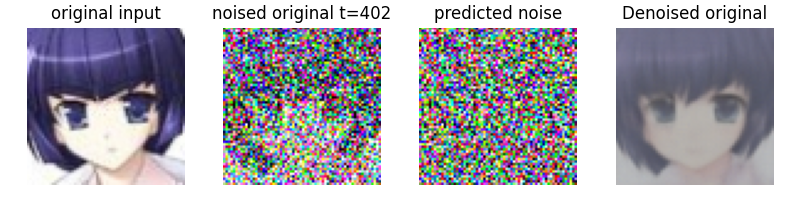
\includegraphics[width=7cm]{figures/media_images_Denoising a sample from validation set_272873_8f570bf75838a8c0f961.png}
    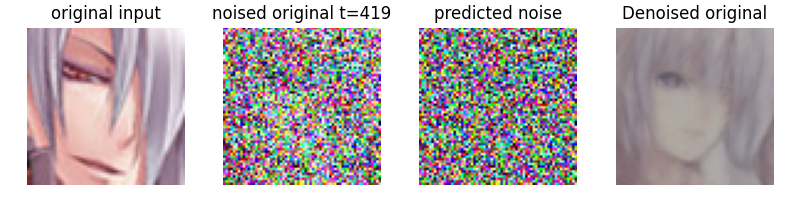
\includegraphics[width=7cm]{figures/media_images_Denoising a sample from validation set_226965_d51d5491ec7767a5c8d0.png}
    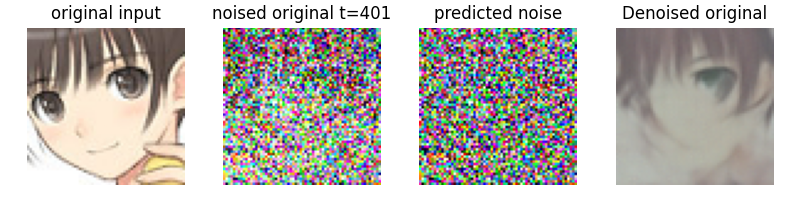
\includegraphics[width=7cm]{figures/media_images_Denoising a sample from validation set_282472_8098099f38ef93fd45ec.png}
    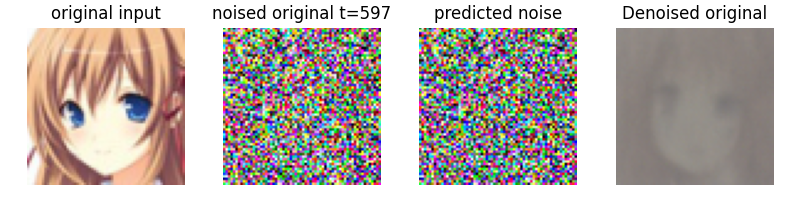
\includegraphics[width=7cm]{figures/media_images_Denoising a sample from validation set_127081_6463e0d9c857dd554363.png}
	\caption{Denoising a sample from validation set for Giga, Mini, Simple and Mega  at step 272873}
	\label{fig:denoising_validation_set}
\end{figure}
the expression to retreive the original image in one step we used is :
$$
 \hat{\mathbf{x}}_0 = \frac{\mathbf{x}_t - \sqrt{1 - \bar{\alpha}_t} \cdot \boldsymbol{\epsilon}_\theta(\mathbf{x}_t, t)}{\sqrt{\alpha_t}}
$$

\subsubsection{Batch Size and Dropout}
\begin{table}[h]
	\centering
	\begin{tabular}{lccc}
		\hline
		Model  & Batch Size & Dropout & learning rate \\
		\hline
		Giga   & 6          & 0.1     & 2e-4          \\
		Mega   & 2          & 0.1     & 2e-4          \\
		Simple & 3          & 0       & 1e-4          \\
		Mini   & 5          & 0       & 1e-4          \\
		\hline
	\end{tabular}
	\caption{Model batch sizes and dropout values}
\end{table}

\subsubsection{Noise Scheduling:}
we used a \textbf{linear scheduler} for the noise $\beta_t$, which is a common choice in DDPMs, as it allows for a smooth transition from low to high noise levels during training. This linear schedule helps the model to learn to denoise images effectively at different noise levels, and it has been shown to work well in practice, It was recommanded to use other strategies like cosine annealing specialy for small datasets, but we estimate that ours is sufficentely large.

\begin{figure}[H]
	\centering
	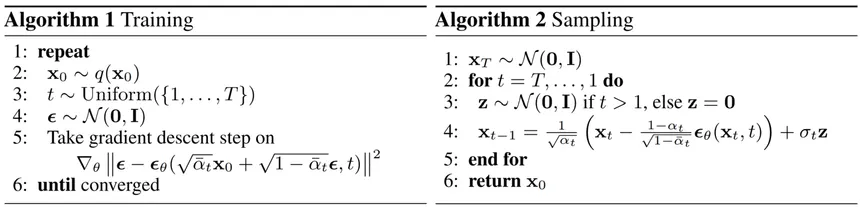
\includegraphics[width=0.45\textwidth]{figures/training-sampling-algo-ddpm.png}
	\caption{training and sampling algorithm for DDPM.}
	\label{fig:train-sampling-algo-ddpm}
\end{figure}

\subsubsection{Parameters}
for learning rate, we trained on $1e-4$ for Mini and Simple, and $2e-4$ for Giga and Mega models.

\subsubsection{Optimizer}
We used the AdamW optimizer, which is an extension of the Adam optimizer with weight decay. AdamW helps to prevent overfitting by adding a weight decay term to the loss function, which dampens oscillations and large gradients.

the desicion to use AdamW was based on its effectiveness in training deep learning models, especially in the context of image tasks. It combines the benefits of adaptive learning rates and weight decay.

we kept the default parameters for AdamW, which are:
\begin{table}[ht]
	\centering
	\begin{tabular}{|c|c|c|c|c|}
		\hline
		$\beta_1$ & $\beta_2$ & $\epsilon$ & weight decay & learning rate \\
		\hline
		0.9       & 0.999     & 1e-8       & 1e-4         & 1e-4          \\
		\hline
	\end{tabular}
	\caption{Optimizer Parameters}
	\label{tab:optimizer_params}
\end{table}

\subsubsection{Loss Function}
the loss function used for training the models is Mean Squared Error. It measures the dissimilarity between the predicted noise and the true noise.
The Mean Squared Error loss is defined as:
\[
	\mathcal{L} = \mathbb{E}_{x \sim p(x), t \sim \mathcal{U}, \epsilon \sim \mathcal{N} } ||(\epsilon - \epsilon_\theta (x_t, t))||^2
\]
we choosed to not consider the upsampling factor in the MSE $\frac{1}{2\sigma_t^2} \frac{(1 - \sigma_t)^2}{(1 - \hat \sigma_t) \sigma_t}$, our goal is not the maximum likelyhood estimation but a better samples.

%%%%%%%%%%%%%%%%%%%%%%%%%%%%%%%%%%%%%% TRAIN/VAL PLOTS %%%%%%%%%%%%%%%%%%%%%%%%%%%%%%%%%%%%%%%%%%%
\begin{figure*}[ht]
	\centering
	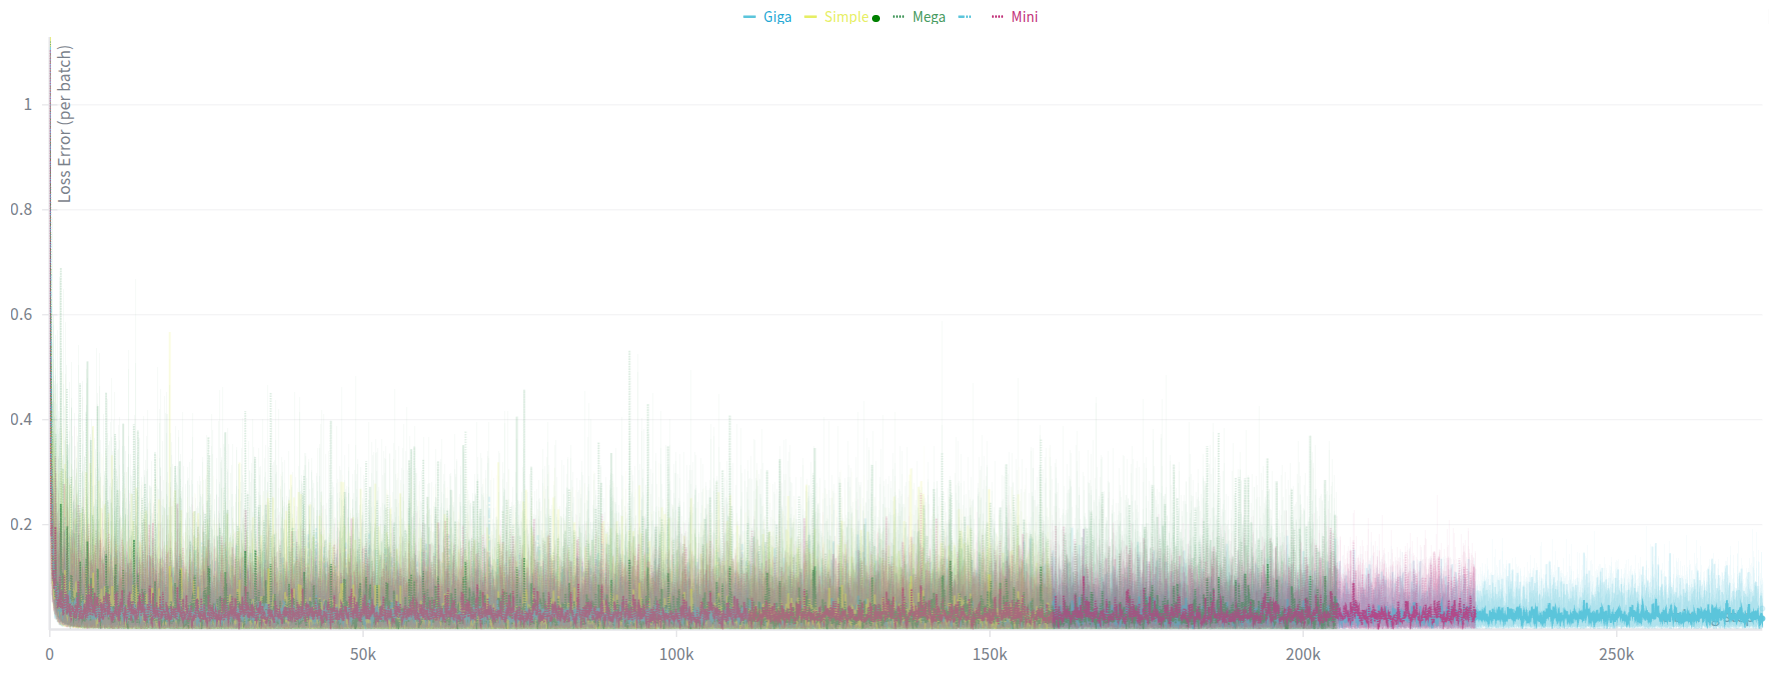
\includegraphics[width=0.9\textwidth]{figures/train----Screenshot from 2025-08-13 19-55-18.png}
	\caption{Evolution of Train Loss per step for each model.}
	\label{fig:train-losses}
\end{figure*}

\begin{figure*}[ht]
	\centering
	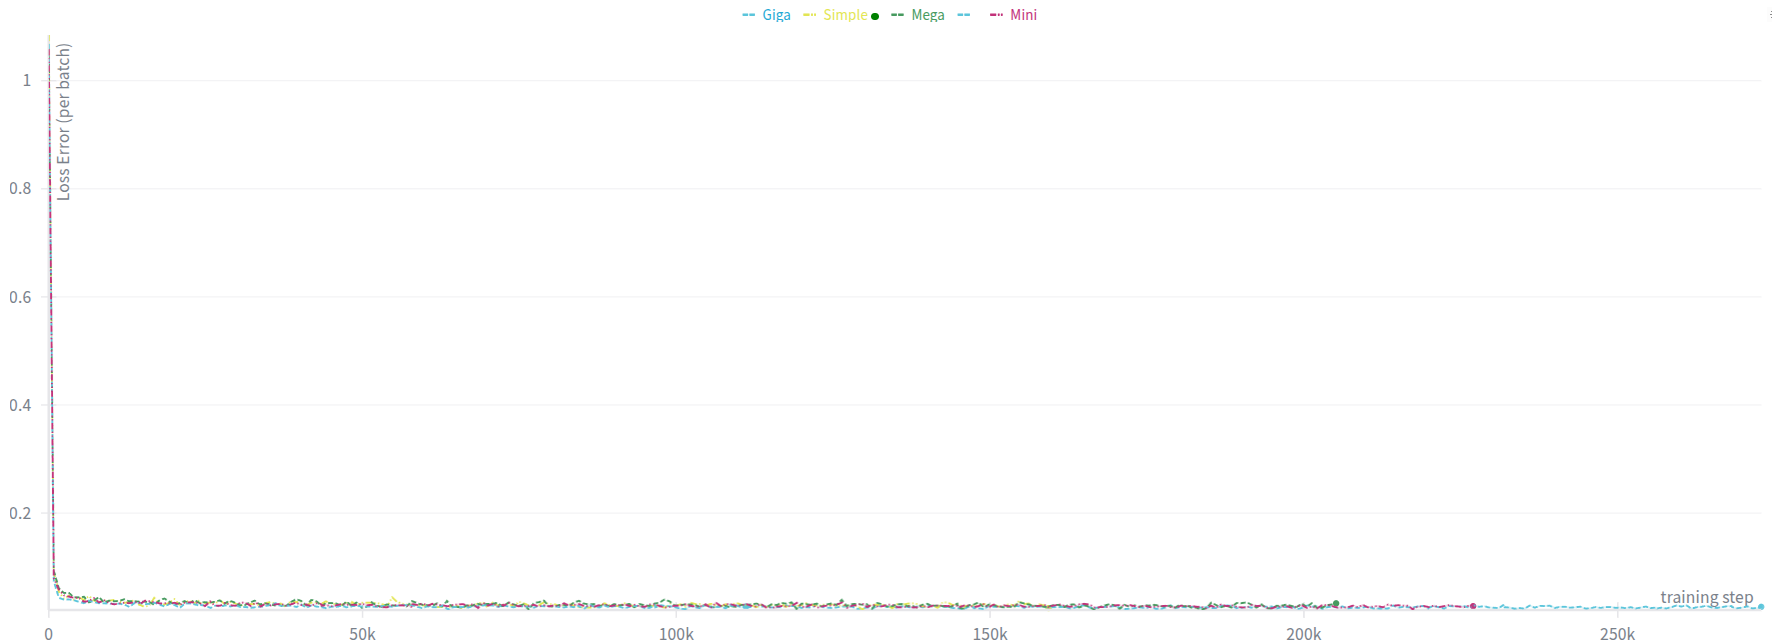
\includegraphics[width=0.9\textwidth]{figures/validation--Screenshot from 2025-08-13 19-56-31.png}
	\caption{Evolution of Validation Loss per step for each model.}
	\label{fig:val-losses}
\end{figure*}
%%%%%%%%%%%%%%%%%%%%%%%%%%%%%%%%%%%%%%%%%%%%%%%%%%%%%%%%%%%%%%%%%%%%%%%%%%%%%%%%%%%%%%%%%%%%%%%%

\section{Results}
Please refer to appendices starting from \ref{tab:mini_10m_bad_attention} to better visualize the results.
%TODO:   one plot (32 samples)for each 3 epochs for each model.


% the bigger the model the faster it learns, it seems contradictory at first, but it can be explained by the increased capacity of larger models to represent complex functions and patterns in the data, because they give more freedom to the model and make it less sensible . This allows them to converge more quickly during training, as they can more easily find and exploit the underlying structure in the data.

% In our case, we found that using attention in the first two block layers of the DownEncoder and UpDecoder was sufficient to achieve good results without significantly increasing the model's complexity.
% , and it seems to be more stable during training, as we can see in the train and validation loss plots.
% as we progress through epochs, small models tend to overfit very fast, 10M and 49M reaches their best generation respectively 1 and 3 but still very low quality, then they tend to denoise images but very low generation quality, while larger models 74M and 85M tend to perform poorly in earlest epochs, and then  generate better quality images respectivly 7 and %TODO but require more data to train and are more sensitive to noise in later time steps.

%mode colapse, althourht 

% having a 
% having the train and validation loss decreasing to very low valaues doies not mean that our generation quality would improve, in contrast, it leads to somtin g siomilar to data colapse in Hierachical VAEs, where the assumption on the distribution of latent variable is too constraining or when the chaining is too short.

% as we can see with the giga model, as we progress in the training the quality improves, but in the Mega models we reach the best generation performence early between the 6th and 7th epochs, an then the quality is contiinously decreasing.

% what we find surprising is the fact that the models with big capacities

% we also a dded a clap for the loss, because we experienced some huge pics in score based model, as the random variable $\epsilon$ can vary unboundely to not breack the assumption of gaussian noise, thethe solution for that is to clip the values of loss error to a certain range.




\section{Discussion} %and future improvements


\subsection{Mode collapse}
As observed in the Mega 74M model, the training process exhibited signs of mode collapse, where the model generated a limited variety of outputs despite having a diverse training dataset. This phenomenon can be attributed to the model's inability to effectively explore the latent space, leading to a convergence towards a few dominant modes despite the model size.
this issue is common for HVAEs, when the assumption on the distribution of latent variable is too constraining or when the chaining is too short, as we can see in the Mega model, as we progress in the training the quality improves, but in the Mega models we reach the best generation performence early between the 6th and 7th epochs, an then the quality is contiinously decreasing.

\subsection{Self-Attention in Unet}
Incorporating self-attention mechanisms into the U-Net architecture enhances its ability to capture long-range dependencies in the input data. This ability to attend to relevant features from distant pixels can be crucial for accurate predictions, and demonstrates the potential of self-attention in tasks requiring contextual understanding even for image generation.

\subsection{Positional Embedding for Self-Attention $\&$ the shape of attention-input}
A possible way to improve the performance of self-attention in our model, could be to explore the use of additional positional embeddings suited for transformer as it wasn't directely imbedded. These embeddings provide the model with information about the relative positions of a set of pixels in the input sequence, which could be used for attention input of the shape $[B, C_i, H*W]$, to allow some subset of pixels attending each others, which is essential for maintaining the spatial structure of the data., instead of making relationships explicit using $[B, H*W, C_i]$.

\subsection{Larger and well structured models learn faster than smaller ones}
As we saw with the shift from Mini 10M to Giga 85M that reached the same generation quality in half the time, thus larger models, due to their increased capacity, can learn more complex patterns and construct richer latent representations faster during training than smaller models, that may struggle to capture the same level of detail. in other word, the larger the model, the more freedom it has to learn complex patterns often without requiring highly precise parameter tuning, which leads to faster convergence and better generalization.

This is impressive for our findings, as it suggests that investing in larger and more sophisticated but well structured models could yield significant improvements in generation quality faster than we thought. and many empirical results support this claim \cite{arora2019finegrained}.

% \subsection{About possible improvements}
%may be if we add a time embeding (positional encoding) specific to attention layers would be better?

% ==============================================================================


% ==============================================================================
\newpage
\bibliographystyle{IEEEtran}
\bibliography{bibliography}
% ==============================================================================

\clearpage
\appendix
% \onecolumn
% \twocolumn[\section*{Appendix}]
\section{The deceptive performance of Score-based Energy model}
We put it as appendix, because we observed very poor performance of the energy distance (ED), with huge fluctuations in the training losses varying from 0.01 to more than 6000, indicating computation instability, see the plot bellow.
\begin{figure}[H]
\centering
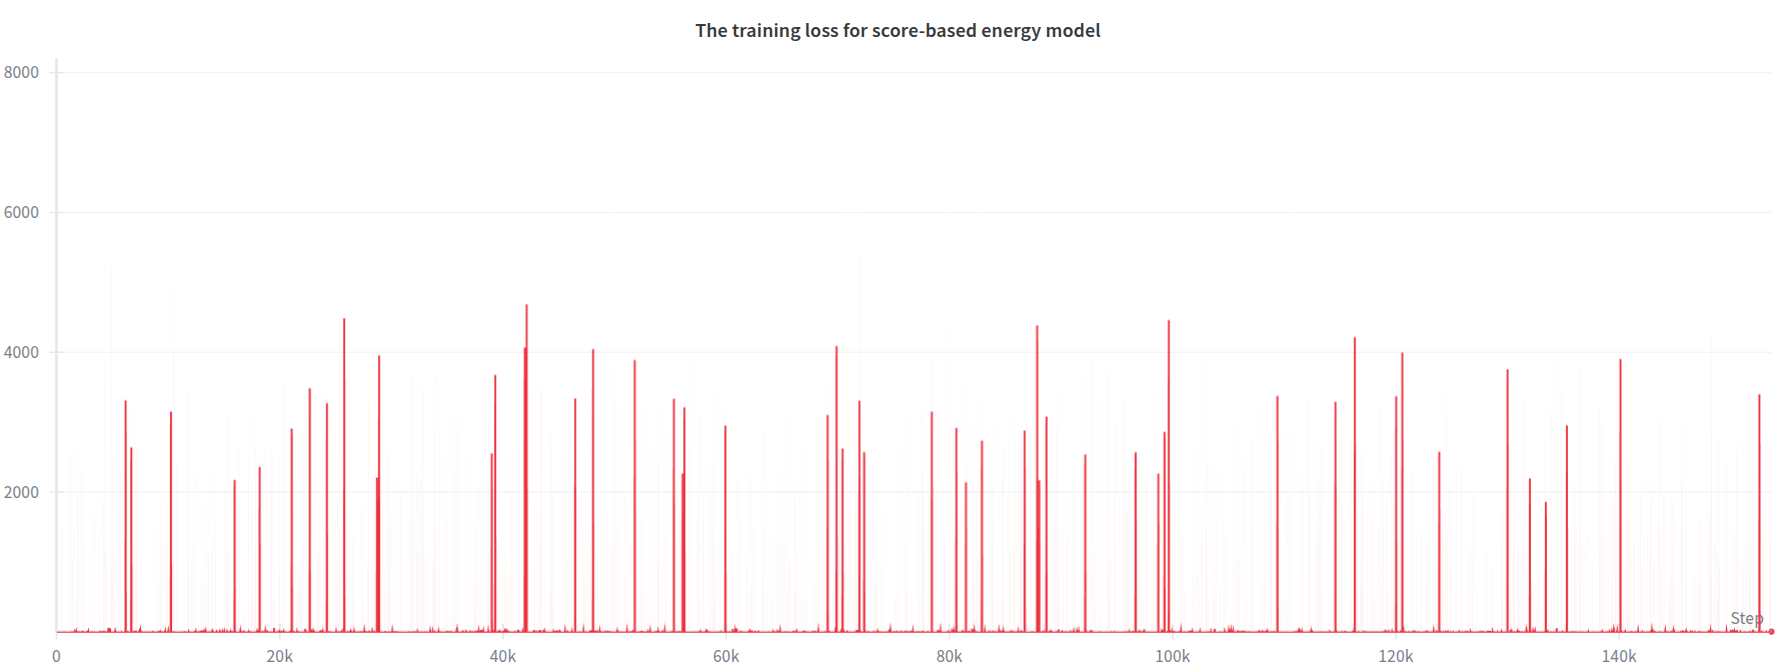
\includegraphics[width=0.5\textwidth]{figures/score-based-loss.png}
\caption{Fluctuations in energy distance (ED) during training.}
\label{fig:energy_distance_fluctuations}
\end{figure}

We attempted to train a score-based energy model following the preconditioning, sampling strategy as well as cosine Scheduling of the paper \cite{karras2022elucidating}, which is a generative model that learns to approximate the score function of the data distribution. The model is trained to predict the score function at different noise levels, and it can generate samples by sampling from the learned distribution.

We also tried to use various steps when sampling, but the result was not satisfactory.

$$
    d\mathbf{x}_t = \left[ -\frac{1}{2} \beta(t) \nabla_{\mathbf{x}} \log p_t(\mathbf{x}) \right] dt + \sqrt{\beta(t)}\, d\mathbf{w}_t
$$
then we approximated this continuous SDE, using the Euler–Maruyama method with step size $\Delta t = 0.01$, in contrast to the paper that proposed higher order Runge-Kutta methods.
$$
    \mathbf{x}_{t - \Delta t} = \mathbf{x}_t + \beta(t) s_\theta(\mathbf{x}_t, t)\, \Delta t + \sqrt{2 \beta(t) \Delta t} \cdot \mathbf{z}, \quad \mathbf{z} \sim \mathcal{N}(0, \mathbf{I})
$$

Refer to the function $q\_sample$ in the notebook $notebooks/0.10-Visualize-samples.ipynb$, which implements the sampling strategy, for the structure of the model refer to $notebooks/2.00-VDM-Score-Energy-based.ipynb$.

\newpage
Here is some samples generated by the model using the above sampling strategy.
\begin{figure}
    \centering
    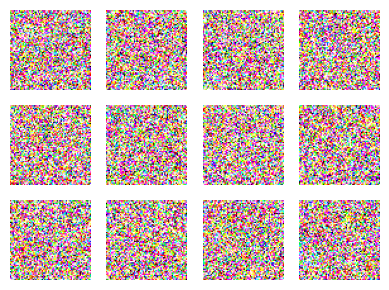
\includegraphics[width=0.5\textwidth]{figures/score-based-sampling.png}
    \caption{Samples generated by the model using the proposed sampling strategy.}
    \label{fig:sample_generated}
\end{figure}

we realise that either we misunderstood the paper, or at least we need to further investigate the training process and the model's architecture to achieve better results. However, we decided to keep our focus on the U-Net architecture and DDPM, as it seems to be more promising for our task.

\newpage

\section{Sampled Images for Mini 10M Architecture}
\begin{figure}[H]
\centering
\begin{tabular}{c|c}
Epoch & Sample Image \\
\hline
2 & 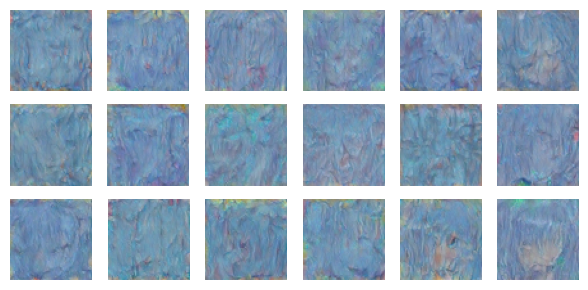
\includegraphics[width=0.3\textwidth]{figures/10M_epoch 2.png} \\
% \hline
5 & 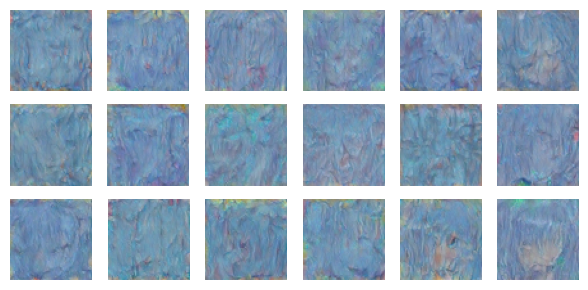
\includegraphics[width=0.3\textwidth]{figures/10M_epoch5_slightely diff_cains_bad_attention_.png} 
\end{tabular}
\caption{Mini 10M epochs with bad attention input shape $[B, C_i, H*W]$.}
\label{tab:mini_10m_bad_attention}
\end{figure}

\begin{figure}[H]
\centering
\begin{tabular}{c|c}
Epoch & Sample Image \\
\hline
1 & 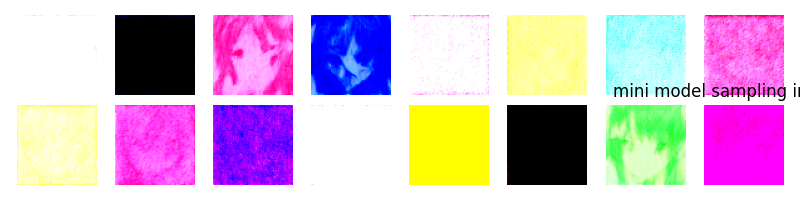
\includegraphics[width=0.42\textwidth]{figures/mini_unet_ddpm_10M_ckpt_epoch_1_epoch_1_samples.png} \\
% \hline
3 & 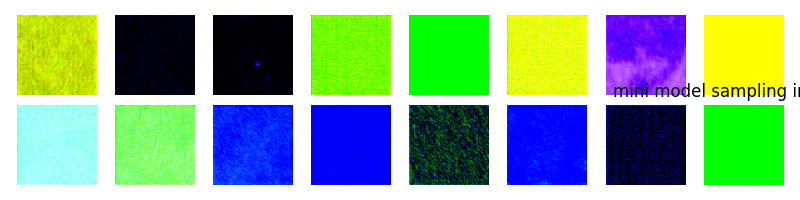
\includegraphics[width=0.42\textwidth]{figures/mini_unet_ddpm_10M_ckpt_epoch_3_epoch_3_samples.png} \\
% \hline
6 & 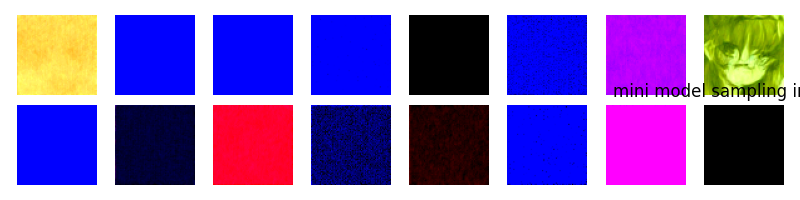
\includegraphics[width=0.42\textwidth]{figures/mini_unet_ddpm_10M_ckpt_epoch_6_epoch_6_samples.png} \\
% \hline
9 & 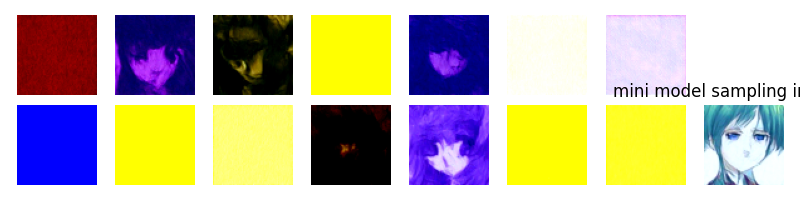
\includegraphics[width=0.42\textwidth]{figures/mini_unet_ddpm_10M_ckpt_epoch_9_epoch_9_samples.png} \\
% \hline
12 & 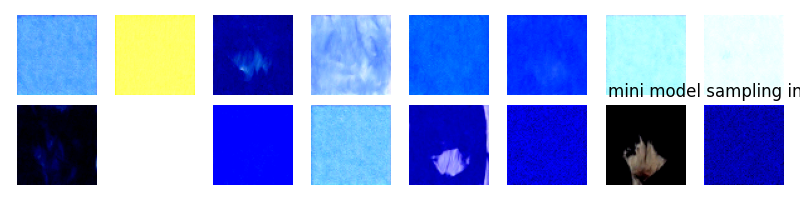
\includegraphics[width=0.42\textwidth]{figures/mini_unet_ddpm_10M_ckpt_epoch_12_epoch_12_samples.png} \\
% \hline
15 & 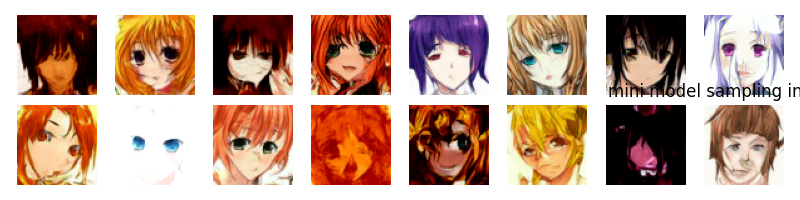
\includegraphics[width=0.42\textwidth]{figures/mini_unet_ddpm_10M_ckpt_epoch_15_epoch_15_samples.png} 
\end{tabular}
\caption{Mini 10M epochs with good attention input shape $[B, H*W, C_i]$}
\label{tab:mini_10m_good_attention}
\end{figure}


\section{Sampled Images for Simple 49M Architecture}
\begin{figure}[H]
\centering
\begin{tabular}{c|c}
\rotatebox{90}{\textbf{Epoch}} & \textbf{Sample Image} \\
\hline
1 & 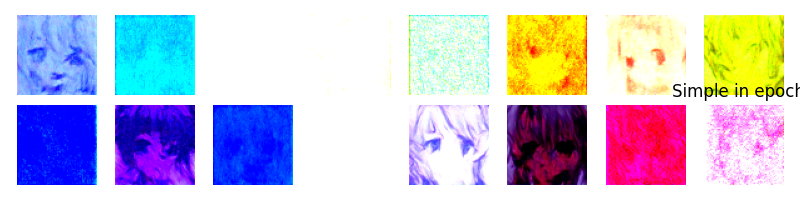
\includegraphics[width=0.42\textwidth]{figures/simple_unet_ddpm_49M_ckpt_epoch_1_2025-08-13_04-50-49_epoch_1_samples.png} \\
% \hline
3 & 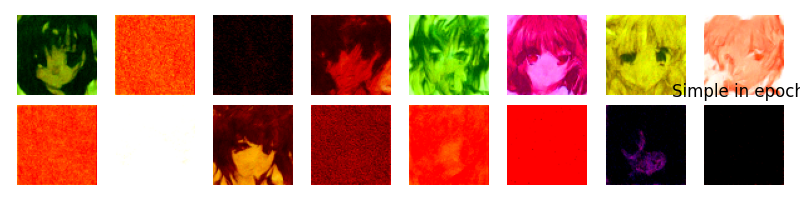
\includegraphics[width=0.42\textwidth]{figures/simple_unet_ddpm_49M_ckpt_epoch_3_2025-08-13_10-10-46_epoch_3_samples.png} \\
% \hline
5 & 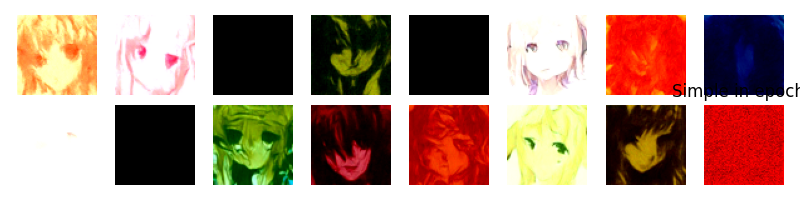
\includegraphics[width=0.42\textwidth]{figures/simple_unet_ddpm_49M_ckpt_epoch_5_2025-08-13_15-33-49_epoch_5_samples.png} \\
% \hline
7 & 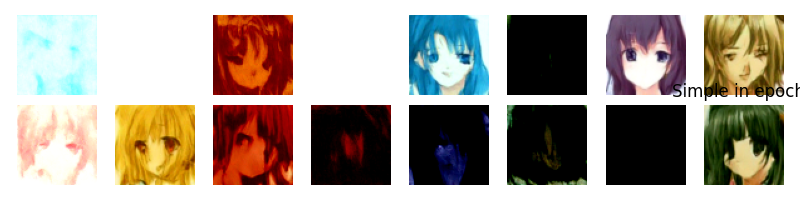
\includegraphics[width=0.42\textwidth]{figures/simple_unet_ddpm_49M_ckpt_epoch_7_2025-08-13_20-54-54_epoch_7_samples.png} \\
% \hline
8 & 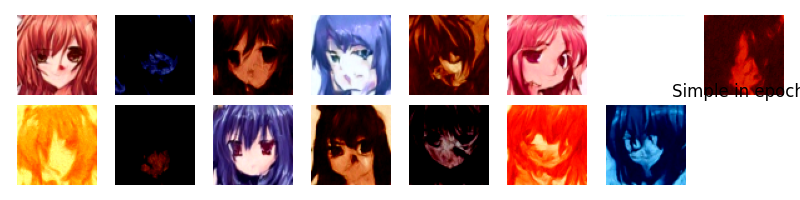
\includegraphics[width=0.42\textwidth]{figures/simple_unet_ddpm_49M_ckpt_epoch_8_2025-08-13_23-35-23_epoch_8_samples.png} \\
% \hline
9 & 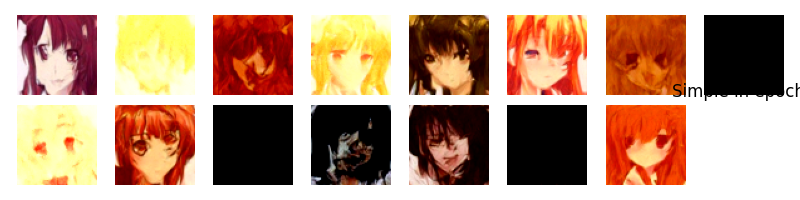
\includegraphics[width=0.42\textwidth]{figures/simple_unet_ddpm_49M_ckpt_epoch_9_2025-08-14_02-15-01_epoch_9_samples.png} \\
% \hline
10 & 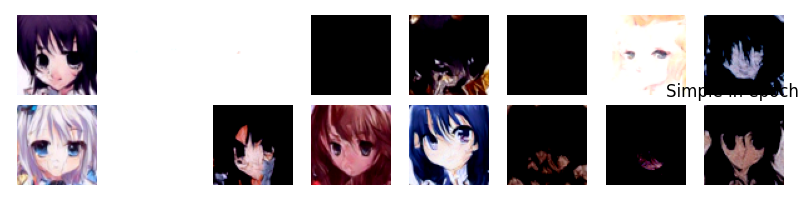
\includegraphics[width=0.42\textwidth]{figures/simple_unet_ddpm_49M_ckpt_epoch_10_2025-08-14_04-54-39_epoch_10_samples.png} \\
% \hline
12 & 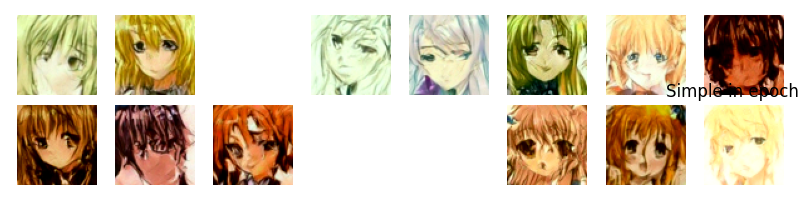
\includegraphics[width=0.42\textwidth]{figures/simple_unet_ddpm_49M_ckpt_epoch_12_2025-08-14_10-13-47_epoch_12_samples.png} \\
% \hline
13 & 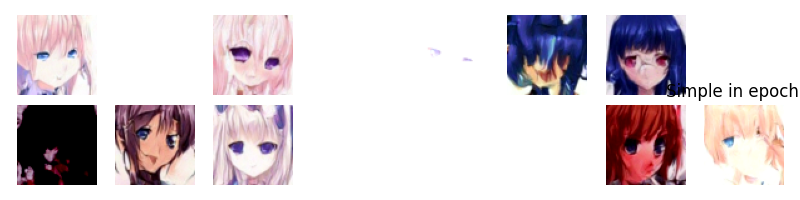
\includegraphics[width=0.42\textwidth]{figures/simple_unet_ddpm_49M_ckpt_epoch_13_2025-08-14_12-52-58_epoch_13_samples.png} 
\end{tabular}
\caption{Simple 49M architecture samples, attention input shape $[B, H*W, C_i]$.}
\label{tab:simple_49m}
\end{figure}

\section{Sampled Images for Mega 74M Architecture:}
\begin{figure}[H]
\centering
\begin{tabular}{c|c}
Epoch & Sample Image \\
\hline
1 & 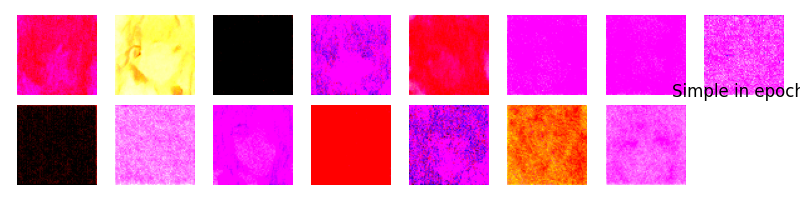
\includegraphics[width=0.42\textwidth]{figures/mega_unet_ddpm_74M_ckpt_epoch_1_epoch_1_samples.png} \\
% \hline
2 & 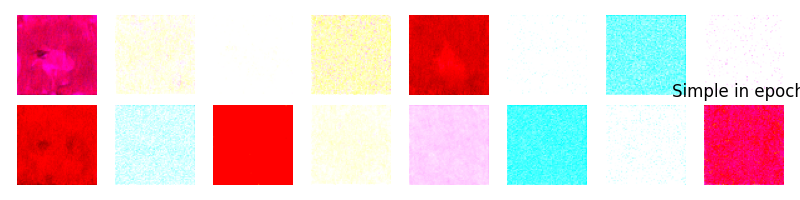
\includegraphics[width=0.42\textwidth]{figures/mega_unet_ddpm_74M_ckpt_epoch_2_epoch_2_samples.png} \\
% \hline
4 & 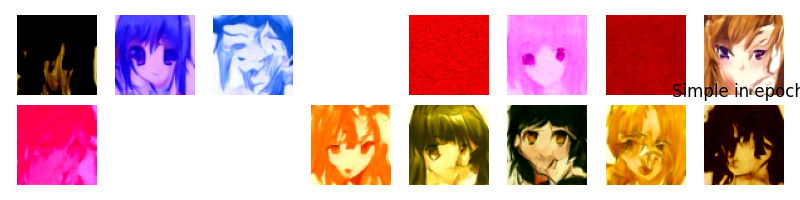
\includegraphics[width=0.42\textwidth]{figures/mega_unet_ddpm_74M_ckpt_epoch_4_epoch_4_samples.png} \\
% \hline
5 & 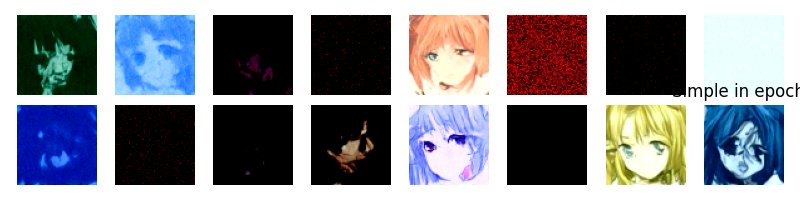
\includegraphics[width=0.42\textwidth]{figures/mega_unet_ddpm_74M_ckpt_epoch_5_epoch_5_samples.png} \\
% \hline
% 16 & 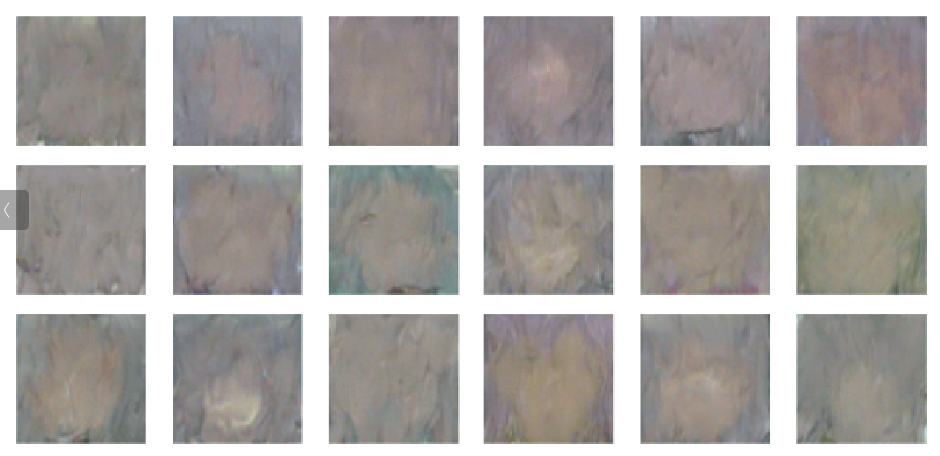
\includegraphics[width=0.42\textwidth]{figures/74M-badattention-epoch16.png} 
\end{tabular}
\caption{Mega 74M architecture samples, attention input shape $[B, H*W, C_i]$.}
\label{tab:mega_74m}
\end{figure}

\section{Sampled Images for Mega 74M Architecture}

\begin{figure}[H]
    \centering
    \label{fig:mega_74m_samples}
    \renewcommand{\arraystretch}{1}
    \setlength{\tabcolsep}{2pt}
    \begin{tabular}{@{}p{0.8cm}|p{0.44\textwidth}@{}}
        \textbf{Epoch} & \textbf{Sample Image} \\
        \hline
        1 & 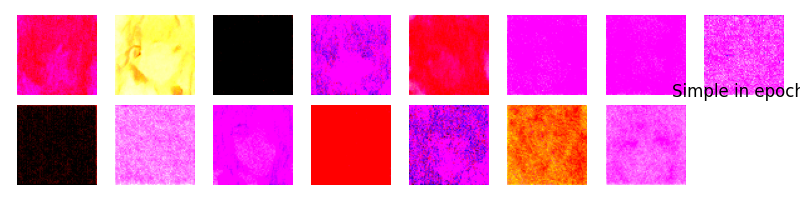
\includegraphics[width=\linewidth]{figures/mega_unet_ddpm_74M_ckpt_epoch_1_epoch_1_samples.png} \\
        2 & 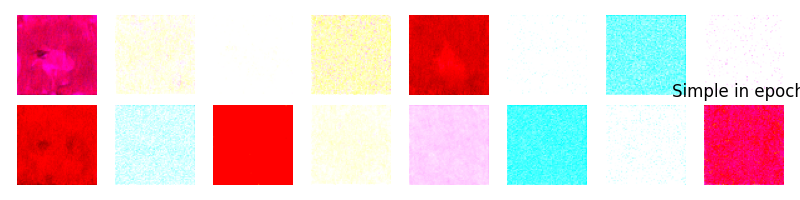
\includegraphics[width=\linewidth]{figures/mega_unet_ddpm_74M_ckpt_epoch_2_epoch_2_samples.png} \\
        4 & 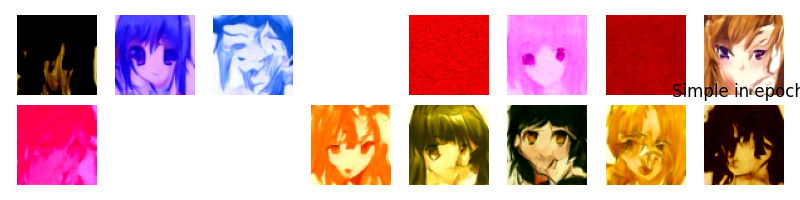
\includegraphics[width=\linewidth]{figures/mega_unet_ddpm_74M_ckpt_epoch_4_epoch_4_samples.png} \\
        5 & 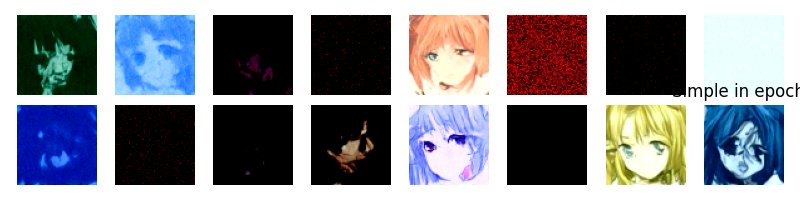
\includegraphics[width=\linewidth]{figures/mega_unet_ddpm_74M_ckpt_epoch_5_epoch_5_samples.png} \\
        % \hline
    \end{tabular}
    \caption{Mega 74M epochs 1, 2, 4 and 5, input shape $[B, H*W, C_i]$.}
\end{figure}


\begin{figure}[H]
    \centering
    \label{tab:mega_74m_samples}
    \begin{tabular}{c|c}
        % \hline
        \textbf{Epoch} & \textbf{Sample Image} \\
        \hline
        1 & \includegraphics[width=0.3\textwidth]{figures/Screenshot from 2025-08-06 09-38-10.png} \\
        2 & \includegraphics[width=0.3\textwidth]{figures/Screenshot from 2025-08-06 09-56-57.png} \\
        4 & \includegraphics[width=0.3\textwidth]{figures/Screenshot from 2025-08-06 12-27-54.png} \\
        % 5 & \includegraphics[width=0.3\textwidth]{figures/Screenshot from 2025-08-06 12-50-24.png} \\
        6 & \includegraphics[width=0.3\textwidth]{figures/Screenshot from 2025-08-06 15-00-11.png} \\
        8 & \includegraphics[width=0.3\textwidth]{figures/Screenshot from 2025-08-06 17-12-05.png} \\
        10 & \includegraphics[width=0.3\textwidth]{figures/Screenshot from 2025-08-06 19-26-11.png} \\
        % 11 & \includegraphics[width=0.3\textwidth]{figures/Screenshot from 2025-08-06 20-09-30.png} \\
        12 & \includegraphics[width=0.3\textwidth]{figures/Screenshot from 2025-08-07 00-02-35.png} \\
        13 & \includegraphics[width=0.3\textwidth]{figures/Screenshot from 2025-08-07 10-10-59.png} \\
        16 & \includegraphics[width=0.3\textwidth]{figures/74M-badattention-epoch16.png} \\
        \hline
    \end{tabular}
    \caption{Mega 74M samples across epochs. Input shape: $[B, C_i, H \times W]$.}

\end{figure}


\section{Sampled Images for Giga 85M Architecture}
\begin{figure}[H]
    \centering
    \caption{Giga 85M samples across selected epochs.}
    \label{tab:giga_85m_samples}
    \renewcommand{\arraystretch}{1} % Reduce row height
    \setlength{\tabcolsep}{2pt}     % Reduce column padding
    \begin{tabular}{@{}p{.3cm}|p{0.41\textwidth}@{}} % Tight Epoch column
        \rotatebox{90}{\textbf{Epoch}} & \textbf{Sample Image} \\
        \hline
        1 & \includegraphics[width=\linewidth]{figures/85M_params_GIGA_DDPM_Unet_ckpt_epoch_1_epoch_1_samples.png} \\
        4 & \includegraphics[width=\linewidth]{figures/85M_params_GIGA_DDPM_Unet_ckpt_epoch_4_epoch_4_samples.png} \\
        5 & \includegraphics[width=\linewidth]{figures/85M_params_GIGA_DDPM_Unet_ckpt_epoch_5_with_16_samples.png} \\
        7 & \includegraphics[width=\linewidth]{figures/85M_params_GIGA_DDPM_Unet_ckpt_epoch_7_epoch_7_samples.png} \\
        9 & \includegraphics[width=\linewidth]{figures/85M_params_GIGA_DDPM_Unet_ckpt_epoch_9.png} \\
        10 & \includegraphics[width=\linewidth]{figures/giga_unet_ddpm_85M_ckpt_epoch_10_epoch_10_samples.png} \\
        13 & \includegraphics[width=\linewidth]{figures/giga_unet_ddpm_85M_ckpt_epoch_13_epoch_13_samples.png} \\
        16 & \includegraphics[width=\linewidth]{figures/giga_unet_ddpm_85M_ckpt_epoch_16_epoch_16_samples.png} \\
        % 17 & \includegraphics[width=\linewidth]{figures/giga_unet_ddpm_85M_ckpt_epoch_17_with_16_samples.png} \\
        % % 19 & \includegraphics[width=\linewidth]{figures/giga_unet_ddpm_85M_ckpt_epoch_19_epoch_19_samples.png} \\
        % 20 & \includegraphics[width=\linewidth]{figures/giga_unet_ddpm_85M_ckpt_epoch_20_epoch_20_samples.png} \\
        % 22 & \includegraphics[width=\linewidth]{figures/giga_unet_ddpm_85M_ckpt_epoch_22_epoch_22_samples.png} 
        % % 19 (Mega variant) & \includegraphics[width=\linewidth]{figures/mega_unet_ddpm_85M_ckpt_epoch_19.png} \\
        % % 22 (Mega variant) &
        %  \includegraphics[width=\linewidth]{figures/mega_unet_ddpm_85M_ckpt_epoch_22_with_16_samples.png} \\
        \hline
    \end{tabular}
\end{figure}

    \begin{figure}[H]
    \centering
    \caption{Giga 85M samples across selected epochs.}
    \label{tab:giga_85m_samples_second_half}
    \renewcommand{\arraystretch}{1} % Reduce row height
    \setlength{\tabcolsep}{2pt}     % Reduce column padding
    \begin{tabular}{|p{.3cm}|p{0.44\textwidth}@{}} % Tight Epoch column
        \rotatebox{90}{\textbf{Epoch}} & \textbf{Sample Image} \\
        \hline
        % 1 & \includegraphics[width=\linewidth]{figures/85M_params_GIGA_DDPM_Unet_ckpt_epoch_1_epoch_1_samples.png} \\
        % 4 & \includegraphics[width=\linewidth]{figures/85M_params_GIGA_DDPM_Unet_ckpt_epoch_4_epoch_4_samples.png} \\
        % 5 & \includegraphics[width=\linewidth]{figures/85M_params_GIGA_DDPM_Unet_ckpt_epoch_5_with_16_samples.png} \\
        % 7 & \includegraphics[width=\linewidth]{figures/85M_params_GIGA_DDPM_Unet_ckpt_epoch_7_epoch_7_samples.png} \\
        % 9 & \includegraphics[width=\linewidth]{figures/85M_params_GIGA_DDPM_Unet_ckpt_epoch_9.png} \\
        % 10 & \includegraphics[width=\linewidth]{figures/giga_unet_ddpm_85M_ckpt_epoch_10_epoch_10_samples.png} \\
        % 13 & \includegraphics[width=\linewidth]{figures/giga_unet_ddpm_85M_ckpt_epoch_13_epoch_13_samples.png} \\
        % 16 & \includegraphics[width=\linewidth]{figures/giga_unet_ddpm_85M_ckpt_epoch_16_epoch_16_samples.png} \\
        17 & \includegraphics[width=\linewidth]{figures/giga_unet_ddpm_85M_ckpt_epoch_17_with_16_samples.png} \\
        \hline
        19 & \includegraphics[width=\linewidth]{figures/giga_unet_ddpm_85M_ckpt_epoch_19_epoch_19_samples.png} 
         \includegraphics[width=\linewidth]{figures/mega_unet_ddpm_85M_ckpt_epoch_19.png} \\
        \hline
        
        20 & \includegraphics[width=\linewidth]{figures/giga_unet_ddpm_85M_ckpt_epoch_20_epoch_20_samples.png} \\
        \hline

        22 & \includegraphics[width=\linewidth]{figures/giga_unet_ddpm_85M_ckpt_epoch_22_epoch_22_samples.png} 
         \includegraphics[width=\linewidth]{figures/mega_unet_ddpm_85M_ckpt_epoch_22_with_16_samples.png} \\
        \hline
    \end{tabular}
\end{figure}


\end{document}